\cleardoublepage{}

\chapter{理论部分}

\section{一些记号}
首先定义一些记号。$\Omega$为数值解区域;
$\partial\Omega=\partial \Omega_D\cup\partial\Omega_N$: 为混合边界条件,例如Dirichlet边界以及Neumann边界条件。
$\mathscr{T}_h$:区域$\Omega$三角化之后离散区域, $h$为衡量标准,例如三角单元最长边。

$\mathscr{E}_h$:  离散化区域$\mathscr{T}_h$中所有边的集合;具体的$\mathscr{E}_h^I$: 离散化区域$\mathscr{T}_h$中内部边的集合, $\mathscr{E}_h^D$: $\mathscr{T}_h\cap\partial\Omega_D $上边的集合,
$\mathscr{E}_h^N$: $\mathscr{T}_h\cap\partial\Omega_N $中边的集合。 
$\mathscr{V}_h$: 离散化区域$\mathscr{T}_h$中所有点的集合。
且记$\tau$ 为离散化区域$\mathscr{T}_h$中一个单元. 

$\Gamma=\partial \Omega$, 
$N_{\mathscr{E}}=card(\mathscr{E}_h),N_v=card(\mathscr{V}_h),N_k=card(\mathscr{T}_h)$, 
$(\cdot,\cdot)$ 和 $<\cdot, \cdot>$ 分别是 $\Omega, \Gamma$ 上的内积记号。


由于我们考虑二维上的问题,因此有必要介绍一些关于向量导数的记号。

粗体字母记号,例如\textbf{u} 代表$u$为一个向量, $(u_1, u_2, \cdots u_n)$, 其中 $n$为定义域维度。 对于 2D, 则有$\textbf{u}=(u_1, u_2)$.\\
那么 $$\nabla \textbf{u}=\begin{pmatrix}
    {u_1}_x & {u_2}_x\\
    {u_1}_y & {u_2}_y
\end{pmatrix}, \nabla \cdot (\nabla \textbf{u})=\Delta \textbf{u}=\begin{pmatrix}
    {u_1}_{xx}+{u_1}_{yy}\\
    {u_2}_{xx}+{u_2}_{yy}\\
\end{pmatrix}$$

为了计算弱形式的方便,我们引入double product:
$$\nabla \textbf{u}:\nabla \textbf{v}=\sum_{j}\sum_{i}\frac{\partial u_i}{\partial x_j}\frac{\partial v_i}{\partial x_j}$$
和索伯列夫空间(Sobolev Space)
$$\begin{aligned}
    H^1(\Omega)&=\{u\in L^2(\Omega):\partial^\alpha u\in L^2(\Omega),|\alpha|\leq 1\}\\
    H^1_0(\Omega)&=\{u\in H^1(\Omega): u|_{\partial \Omega}=0\}\\
    L^2_0(\Omega)&=\{u\in L^2(\Omega): \int_\Omega u=0\}
\end{aligned}$$

对于向量 $\textbf{u}\in [H^1_0]^n$, 
有范数 $$\left\|\textbf{u}\right\|_{H^1_0}=\left(\left\|\textbf{u}\right\|^2_{L^2(\Omega)}+\left\|\nabla \cdot \textbf{u}\right\|^2_{L^2(\Omega)}\right)^{\frac{1}{2}}$$

接下来研究经典数值算法中的间断Galerkin方法。


\section{间断有限元方法(Discontinuous Galerkin Method)}\label{Interior Penalty Discontinuous Galerkin Method}
间断有限元方法\cite{DGM}是属于有限元类的数值方法,大致思路和一般有限元方法类似,选取基函数,最后求解为基函数的线性表示。最先被设计用于解决双曲守恒定律的经典数值算法,在近些年里逐渐变得流行。
其主要特点在于允许解有间断性,这在解决拥有间断,突变解的问题上有着很大的优势。

我们选择间断有限元方法主要是由于它以下灵活性:
\begin{itemize}
    \item 允许利用任意已知点,在任意区域内进行三角划分
    \item 在每个单元上可以自由的选择用于拟合的多项式的次数
    \item 可以实现很高效率的并行计算 
\end{itemize}

间断有限元方法也有很多方式,如内罚间断,局部间断以及杂交间断等方式\cite{numpde}。在这里我们主要研究内罚间断有限元方法(Interior Penalty Discontinuous Galerkin Method),并以解决Possion方程为例。

首先因为DG方法本身允许解的间断,有如下定义:

\begin{definition}[Jump and average]
    定义边上跳量和平均量:
    $$\left\{
    \begin{aligned}
        &[u]_{kl}=(u|_{\tau_k}-u|_{\tau_l})\\
        &{u}= \frac{1}{2}(u|_{\tau_k}+u|_{\tau_l})
    \end{aligned}
\right.$$
其中kl为边$e\in \mathscr{E}^I$邻居单元k和单元l。

若$e\in \mathscr{E}^D$,只有邻居单元k,则定义为
$$\left\{\begin{aligned}
    &[u]_{k}=u|_{\tau_k}\\
    &{u}= u|_{\tau_k}
\end{aligned}\right.$$
\end{definition}


\begin{definition}[Broken Sobolev space]
    对于  $p \geq 0$  Broken Sobolev space为
    $$H^{p}\left(\mathscr{T}_h\right):=\left\{v \in L_{2}(\Omega): v|_{\tau} \in H^{p}\left(\tau\right) \text { for all } \tau \in \mathscr{T}_h\right\}$$
    有分片p阶多项式组成的离散函数空间为
    $$S^p_h(\mathscr{T}_h):=\{v_h\in L_2(\Omega):v_h|_{\tau}\in\mathbb{P}_p(\tau),\forall \tau \in \mathscr{T}_h\}$$
\end{definition}

限制在 $\tau \in \mathscr{T}_h$ 属于索伯列夫空间 并且在$\tau$的内部边界上可以不连续。

\subsection{Possion方程}
考虑有混合边界的Possion方程,介绍其理论框架。首先Possion方程有如下形式:
\begin{equation}\label{possion}
    \left\{\begin{aligned}
    &-\nabla\cdot(a(\nabla u))=f\qquad x \in \Omega\\
    &u=g_D \qquad x\in\Gamma_D\\
    &u=g_N \qquad x\in\Gamma_N
\end{aligned}\right.\end{equation}

在这里我们假设 $g_D=0$. 我们将其画为弱解形式: 对于 $\forall v\in V:=\{v|_\tau\in H^2(\tau),\forall \tau\in \mathscr{T}_h\}$
\begin{equation}\label{1-2}
    \begin{aligned}
    (f, v) & =-\int_{\Omega} \nabla \cdot(a \nabla u) v=-\sum_{\tau \in \mathscr{T}_{h}} \int_{\tau} \nabla \cdot(a \nabla u) v \\
    & =\sum_{\tau \in \mathscr{T}_{h}} \int_{\tau} a \nabla u \cdot \nabla v-\sum_{\tau \in \mathscr{T}_{h}} \int_{\partial \tau} a \textbf{n}_{\tau}\cdot \nabla u  v .
    \end{aligned}
\end{equation}
先补充一个定理:
\begin{theorem}(\textbf{Sobolev Embedding Theroem})
    若 $u\in W^{k,p}(\Omega)$, 其中 $p>1$, 当 $m:=k-\frac{n}{p}>0$, 那么 $u\in C^{m}(\Omega)$
\end{theorem}

因此由上述定理,如果 $u\in H^2(\Omega)$, 所以 $u\in C^m(\Omega)$,即 $[u]=[\nabla u]=0$

因此式子(\ref{1-2})的右边第二项可以写成:
$$\begin{aligned}
\sum_{\tau \in \mathscr{T}_{h}} \int_{\partial \tau} a & \nabla u \cdot \textbf{n}_{\tau} v=\sum_{e \in \mathcal{E}_{h}^{I}} \int_{e}[a \textbf{n}\cdot \nabla u  v] +\sum_{e \in \mathcal{E}_{h}^{D}} \int_{e} a\textbf{n}\cdot \nabla u  v + \sum_{e \in \mathcal{E}_{h}^{N}} \int_{e} a \textbf{n}\cdot \nabla u  v \\
& =\sum_{e \in \mathcal{E}_{h}^{I}} \int_{e}([a \nabla u \cdot \textbf{n}]\{v\}+\{a \nabla u \cdot \textbf{n}\}[v])+\sum_{e \in \mathcal{E}_{h}^{D}} \int_{e} a \nabla u \cdot \textbf{n} v +\int_{\Omega_N}g_Nv\\
& =\langle\{a \nabla u \cdot \textbf{n}\},[v]\rangle_{\mathcal{E}_{h}^{I D}}+\int_{\Omega_N}g_Nv
\end{aligned}$$

所以(\ref{1-2})可以有形式:
\begin{equation}\label{1-3}
    (a \nabla u, \nabla v)_{\mathscr{T}_{h}}-\langle\{a \nabla u \cdot \textbf{n}\},[v]\rangle_{\mathcal{E}_{h}^{I D}}=(f, v)_{\mathscr{T}_h}+\int_{\Omega_N}g_Nv, \quad \forall v \in V .
\end{equation}

为了最后刚度矩阵对称性考虑,添加对称项,对称系数为$\epsilon$。同时我们可以发现(\ref{1-3})中其实没有涉及边界条件,因此添加用于约束边界的惩罚项,惩罚因子为$\sigma$。

于是我们可以定义双线性型:

$$\left\{\begin{aligned}
    &A_{h}(u, v):=  (a \nabla u, \nabla v)_{\mathscr{T}_{h}}-\left(\langle\{a\textbf{n}\cdot \nabla u \},[v]\rangle_{\mathcal{E}_{h}^{I D}}-\epsilon\langle\{a \textbf{n}\cdot\nabla v \}, [u]\rangle_{\mathcal{E}_{h}^{I D}}\right)+J_{0}(u, v)+J_{1}(u, v)\\
    &F_h(v)=(f, v)_{\mathscr{T}_h}+\int_{\Omega_N}g_Nv+\epsilon\langle\{a \textbf{n}\cdot\nabla v \}, [u]\rangle_{\mathcal{E}_{h}^{D}}, \quad \forall v \in V
\end{aligned}\right.$$
其中 $$J_{0}(u, v):= \sum_{e \in \mathcal{E}_{h}^{I D}} \frac{\sigma_{0}}{h_{e}} \int_{e}[u][v],\qquad
J_{1}(u, v):= \sum_{e \in \mathcal{E}_{h}^{I}} \sigma_{1} h_{e} \int_{e}[a \nabla u \cdot n][a \nabla v \cdot n]$$

注意到对于精确解 $u$ 而言,我们自然的有 
$$\left\{\begin{aligned}
    &\epsilon\langle\{a \textbf{n}\cdot\nabla v \}, [u]\rangle_{\mathcal{E}_{h}^{I D}}=\epsilon\langle a \textbf{n}\cdot\nabla v, u\rangle_{\mathcal{E}_{h}^{D}}\\
    &J_{0}(u, v)= \sum_{e \in \mathcal{E}_{h}^{D}} \frac{\sigma_{0}}{h_{e}} \int_{e}g_Dv\\
    &J_1(u,v) = 0
\end{aligned}\right.$$

因此我们需要找到 $ u_{h} \in S_h^p(\mathscr{T}_h)$ s.t.

\begin{equation}\label{dgpossion}
    A_{h}\left(u_{h}, v_{h}\right)=F_h(v_h) \quad \forall v_{h} \in S_h^p(\mathscr{T}_h) .
\end{equation}

这里我们仅考虑拥有齐次边界条件的精确解 $u$来说, 我们显然有
$$\langle\{a \nabla v \cdot n\},[u]\rangle_{\mathcal{E}_{h}^{I D}}=J_{0}(u, v)=J_{1}(u, v)=0, \quad \forall v \in V$$


之后我们只需要像平常的有限元方法一样寻找基函数即可。
例如我们设$u_h=\sum_{i=1}^{N_h}u_i\phi_i$, 那么 
$$\sum_{j=1}^{N_h}A_h(\phi_j,\phi_i)u_j=F_h(\phi_i),i=1\cdots N_h$$
这可以被写作为矩阵形式 $AU=F$

因此上边所离散的问题等价于一个线性方程组的问题,我们可以通过选择合适的方法解决。并且可以注意到矩阵A为稀疏矩阵,
当单元数量变多时,网格大小变为$(Nloc\times Nelt)^2$。

\subsubsection*{\textbf{注:}}
    在这里考虑到矩阵的稀疏性,其实有一些工作针对与稀疏矩阵的处理,无论是经典的数值算法还是深度学习方法。

    经典的数值算法例如多重网格方法用来加速矩阵运算。
    深度学习方法近些年有些工作专注于利用图神经网络进行加速求解,因为图结构所构成的邻接矩阵同样是大型稀疏的,之间非常相似。
    那么如何将图神经网络和有限元中的稀疏关系结合从而相辅相成是一个值的思考的问题。

接下来我们考虑关于求解瞬态PDE方程的特殊方法。
\section{瞬态问题(Time-dependent problems)}
关于稳态方程,也即时间无关的偏微分方程,我们在很大程度上有很多手段处理。但是一旦涉及到时间项,如何处理解随时间动态变化的问题开始变得棘手起来。并且时间项处理的好坏直接影响着结果的优劣,一些经经常出现的问题如误差累积,以及并行计算的困难等等。

事实上我们主要有三种方法解决瞬态问题。
\begin{itemize}
    \item 对于时间项,使用差分方法,如单步法,线性多步法,来进行时间步长迭代。
    \item 空间维度用有限元方法进行离散,最后将PDE系统化为为ODE系统,之后解关于ODE系统方程组。
    \item 利用时空有限元方法(STFEM)同时离散空间和时间维度;
\end{itemize}

基于NS方程在下面几部分中分别讨论了这三种方法。在这里,我们仅考虑其次Dirichlet边界条件,$\Omega$ 为空间区域,$I=(0,T)$ 为时间域,方程可以写作为:
$$\left\{
    \begin{aligned}
        &\textbf{u}_t+(\textbf{u}\cdot \nabla)\textbf{u}+\frac{1}{\rho}\nabla p-\gamma \Delta \textbf{u}=\textbf{f}\quad \text{in} \ \Omega\times I\\
        &\nabla \cdot \textbf{u}=0\\
        &\textbf{u}|_{\partial \Omega}=0
    \end{aligned}
\right.$$

\subsection{时间差分}
首先我们尝试时间差分离散化。我们通常有高效并且成熟的数值方法来处理时间项,如龙格库塔方法。
以向前欧拉方法(Forward Euler Method)为例子,我们有
\begin{equation}
    \begin{aligned}
    &\frac{\textbf{u}_{n+1}-\textbf{u}_n}{\Delta t}=\gamma \Delta \textbf{u}_n-(\textbf{u}_n\cdot \nabla) \textbf{u}_n-\frac{1}{\rho}\nabla p_n+\textbf{f}\stackrel{\text{denote}}{=}\textbf{F}(\textbf{u}_n,p_n)\\
    \Rightarrow&\textbf{u}_{n+1}=\textbf{u}_n+\Delta t \textbf{F}(\textbf{u}_n,p_n)
    \end{aligned}  
    \label{1}
\end{equation}

其中 $\textbf{u}_n$ 代表在第n步的解 $\textbf{u}$,可以看到该方法主要以迭代的方式进行时间步长的推演。
当然也有其他时间离散方案如 leapfrog method, RK method等等,分为显式和隐式方法。 

然而由于 $\textbf{u}_{n+1}$ 可能不满足 $\nabla \cdot \textbf{u}=0$ 并且没有办法处理压力项 $p_n$. 
因此对于NS方程需要引入 Splitting Operator Method。方法如下:

通常我们同时有 
\begin{equation}
    \frac{\textbf{u}_{n+1}-\textbf{u}_n}{\Delta t}=\gamma \Delta \textbf{u}_n-(\textbf{u}_n\cdot \nabla) \textbf{u}_n-\frac{1}{\rho}\nabla p_{n+1}+\textbf{f}=\textbf{F}(\textbf{u}_n,p_{n+1})\\
\end{equation}
其中 $\nabla \cdot \textbf{u}_{n+1}=0$. 并且我们记 (\ref*{1})中$\textbf{u}_{n+1}$  为 $\textbf{u}^*$. 

那么我们需要寻找一个修正 $\delta \textbf{u}$ s.t. $\textbf{u}_{n+1}=\textbf{u}^*+\delta \textbf{u}$。

因此
 $$\delta \textbf{u}=-\frac{\Delta t}{\rho}\nabla(p_{n+1}-\beta p_n)\stackrel{denote}{=}-\frac{\Delta t}{\rho}\nabla \Phi$$
i.e. $\Phi=p_{n+1}-p_n$. 

代入$\nabla\cdot \textbf{u}_{n+1}=\nabla \cdot(\textbf{u}^*+\delta \textbf{u})=\nabla \cdot (\textbf{u}^*-\frac{\rho}{\Delta t}\nabla\Phi)=0$, 
也即
\begin{equation}
    \Delta \Phi = \frac{\rho}{\Delta t}\nabla \cdot \textbf{u}
    \label{Possion}
\end{equation} 

然后我们可以更新 $\textbf{u}_{n+1},p_{n+1}$, 通过 
\begin{equation}\label{2-4}\left\{
    \begin{aligned}
        &\textbf{u}_{n+1}=\textbf{u}^*-\frac{\Delta t}{\rho}\nabla \Phi\\
        &p_{n+1}=\Phi + \beta p_n
    \end{aligned}\right.
\end{equation}

这是一种将复杂问题转化为简单的小问题的方法。
\begin{tcolorbox}
    总结步骤如下:
    \begin{itemize}
        \item 计算 $\textbf{u}^*$
        \item 解一般Possion方程 (\ref*{Possion})
        \item 根据(\ref{2-4})更新 $\textbf{u}_{n+1}$\&$p_{n+1}$
    \end{itemize}
\end{tcolorbox}


随后我们推导弱解形式。引入测试函数$\textbf{v}^{(u)}\in V^{(u)}$\& $\textbf{v}^{(\phi)}\in V^{(\phi)}$。
由分部积分可以得到如何两项的逼近形式:
$$\begin{aligned}
    &\int_\Omega\Delta \textbf{u}\textbf{v}=-\int_\Omega\nabla\textbf{u}:\nabla\textbf{v}+\int_{\partial\Omega}\frac{\partial \textbf{u}}{\partial \textbf{n}}\cdot \textbf{v}ds\\
    &\int_\Omega \nabla p\cdot \textbf{v}=-\int_\Omega p\cdot \nabla \cdot \textbf{v}+\int_{\partial \Omega}p\cdot\textbf{n}\textbf{v}ds
\end{aligned}$$
其中 $\frac{\partial \textbf{u}}{\partial \textbf{n}}=\textbf{n}\cdot \nabla \textbf{u}$。
因此我们得到弱解形式为
\begin{equation}
    \begin{aligned}
        &\int_\Omega\left[\textbf{u}^*\textbf{v}^{(u)}+\Delta t(\textbf{u}_n\cdot \nabla)\textbf{u}_n\cdot \textbf{v}_n\right]-\int_\Omega\beta \frac{\Delta t}{\rho}p^n\nabla\cdot \textbf{v}^{(u)}
        +\int_\Omega \Delta t\gamma \nabla\textbf{u}_n:\nabla \textbf{v}_n\\
        &=\int_\Omega\Delta t \gamma \textbf{f}\cdot \textbf{v} + \int_\Omega\left(\Delta t\gamma\frac{\partial \textbf{u}}{\partial \textbf{n}}\textbf{v}^{(u)}-\beta\frac{\Delta t}{\rho}p\cdot\textbf{n}\textbf{v}\right)ds\\
        &\int_{\Omega} \nabla \Phi\cdot \nabla \textbf{v}^{\phi}=-\frac{\rho}{\Delta t}\int_\Omega \nabla \cdot \textbf{u}^*\cdot \textbf{v}^{(\phi)}+\int_{\partial\Omega}\frac{\partial \Phi}{\partial \textbf{n}}\textbf{v}^{(\phi)}ds
    \end{aligned}
\end{equation}

但是这种方法的缺陷是容易造成误差累计,并且需要很强的稳定性条件。因此我们需要更多的连续性,更好的离散性。

\subsection{转化为ODE系统}
我们可以直接得到NS方程的弱解形式:
\begin{equation*}\left\{
    \begin{aligned}
        &\int_\Omega \textbf{u}_t \textbf{v} + \int_\Omega \gamma \nabla \textbf{u}:\nabla\textbf{v} + \frac{1}{\rho}\int_\Omega p\nabla \cdot\textbf{v}+\int_\Omega(\textbf{u}\cdot \nabla) \textbf{u}\cdot\textbf{v}\\
        &=\int_\Omega \textbf{f}\cdot\textbf{v}+ \int_\Omega\left(\gamma\frac{\partial \textbf{u}}{\partial \textbf{n}}\textbf{v}^{(u)}-\frac{1}{\rho}p\cdot\textbf{n}\textbf{v}\right)ds\qquad &\textbf{v}\in V\\
        &\int_\Omega \nabla\cdot \textbf{u} q=0 &q\in W
    \end{aligned}\right.
\end{equation*}

用记号可以化简为

\begin{equation*}\left\{
    \begin{aligned}
        &(\textbf{u}_t, \textbf{v})+\gamma a(\textbf{u}, \textbf{v})-\frac{1}{\rho}b(\textbf{v}, p)+((\textbf{u}\cdot \nabla)\textbf{u}, \textbf{v})=(\textbf{f}, \textbf{v})\\
        &b(\textbf{u}, q)=0
    \end{aligned}\right.
\end{equation*}

设离散化函数空间 $V_h\subset V, W_h\subset W$ 的基函数分别为为 $\{\phi_1, \phi_2,\cdots \phi_{N_v}\}$ ,因此可以设 $$u^h=\sum_{i=1}^{N_v}U(t,\textbf{x}_i)\phi_i(\textbf{x})$$ 

代入到弱形式中可以得到
\begin{equation*}\left\{
    \begin{aligned}
        &(\textbf{u}^h_t, \textbf{v}^h)+\gamma a(\textbf{u}^h, \textbf{v}^h)-\frac{1}{\rho}b(\textbf{v}^h, p^h)+((\textbf{u}^h\cdot \nabla)\textbf{u}^h, \textbf{v}^h)=(\textbf{f}, \textbf{v}^h)\\
        &b(\textbf{u}^h, q^h)=0
    \end{aligned}\right.
\end{equation*}

那么可以将方程转化为ODE系统。但是我们可以发现非线性项非常难处理。需要用类牛顿迭代等方法进行迭代计算。因此我们提出第三种方法时空方法。

\section{时空有限元(Space-Time FEM)}
第三种方法研究了时空有限元方法\cite{STM}。这里的时空方法主要是指将时间维度作为最后一维加入到定义域中。这种方法最大的一个优点是他们可以自然的处理一些有关动边界的问题。另一个优点是在处理有局部奇点问题有很大优势。
缺点也很容易发现,很容易陷入维度灾难。 当问题涉及到三维之后,添加时间维度之后,定义域变成四维空间,数值计算变得非常复杂。但这提供了一种不同的看待时间维度的方法。

在这里我们首先主要介绍基于间断有限元的时空方法,并给出相关的误差以及收敛性分析。
简单点来说,它和普通的有限元方法相比最大不同,就在于它的目标是寻找一组依赖于时间的基函数${\phi_i(t,x)}$的线性组合。
首先基于热方程,介绍时空有限元方法的方案原理,随后基于NS方程再给出方案的理论分析。

\subsection{热方程}
第一个模型我们基于拥有混合边界条件的热方程,其数学形式如下所示:
$$\left\{\begin{aligned}
&c  u_t(\textbf{x}, t)-\nabla_x \cdot\left[A(\textbf{x}, t) \nabla_x u(x, t)\right]  =f(\textbf{x}, t) & \text { for }(\textbf{x}, t) \in Q:=\Omega \times(0, T), \\
&u(\textbf{x}, t) =g_D  & \text { for }(\textbf{x}, t) \in \Sigma_D:=\Gamma_D \times(0, T), \\
&\textbf{n}_x\cdot \nabla_xu=g_N & \text{ for } (\textbf{x}, t) \in \Sigma_N:=\Gamma_N \times(0, T)\\
&u(\textbf{x}, 0) =u_{0}(\textbf{x})  & \text { for } \textbf{x} \in \Omega,
\end{aligned}\right.$$

其中  $A(\textbf{x}, t)=[A(\textbf{x}, t)]^{\top} \in \mathbb{R}^{n \times n}$为系数,在  $(\textbf{x}, t) \in Q $为正定矩阵形式,通常情况下我们将其设为I; 
$c>0$ 为热容常数,通常将其当作常数1, T 为给定的模拟结束时间。$f \in L_{2}\left(0, T\right)$是给定的热源项。我们假设 $u_{0} \in H^{1}(\Omega)$.

\subsubsection*{时空区域离散}
记Q(1D)为2D时空区域,即空间区域为1维,时间作为第二维度,如下图所示

\begin{center}
    \begin{tikzpicture}
        \draw[->, thick] (-1,0) -- (5,0) node[right] {$x$};  
        \draw[->, thick] (0,-1) -- (0,5) node[above] {$t$};
        \draw (0,0)--(4,0)--(4,4)--(0,4)--(0,0);
        \node at (2,4.5) {$\Sigma_T$};
        \node at (4.5,2) {$\Sigma_N$};
        \node at (-0.5,2) {$\Sigma_D$};
        \node at (2,-0.5) {$\Sigma_0$};
        \node at (4,-0.5) {$X$};
        \node at (-0.5,4) {$T$};
        \node at (2,2) {$Q$};
    \end{tikzpicture}
\end{center}

%   \cap H^{1}(0, T, H^{-1}(\Omega))
在这里我们只考虑纯Dirichlet边界条件。

这里的离散方法和DG方法种类似,但其实可以对区域进行广义离散,如图\ref{fig},这在处理动边界问题时有很大的优势。

\begin{figure}[H]
    \begin{center}
        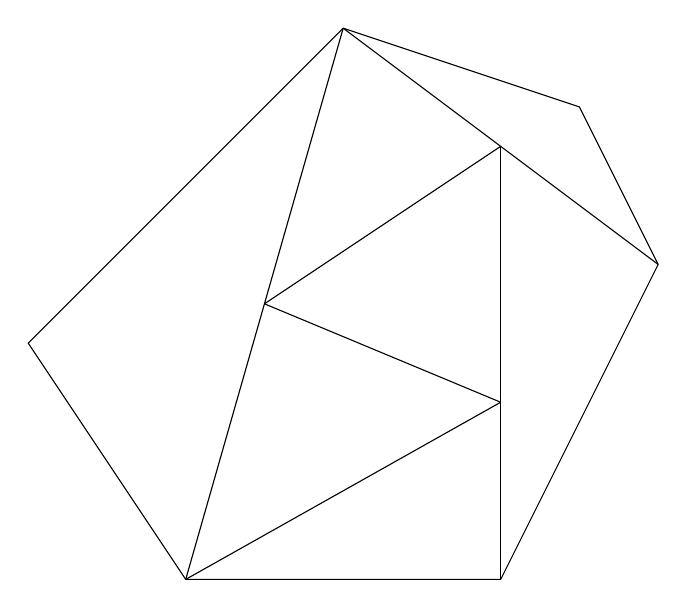
\begin{tikzpicture}
            \draw (0,0)--(4,0)--(6,4)--(5,6)--(2,7)--(-2, 3)--(0,0);
            \draw (0,0)--(2,7);
            \draw (1, 3.5)--(4,5.5);
            \draw (2, 7)--(6,4);
            \draw (4,5.5)--(4,0);
            \draw (4, 2.25)--(1,3.5);
            \draw (0,0)--(4, 2.25);
    
        \end{tikzpicture}
    \end{center}
    \caption{广义离散}  
    \label{fig}  
\end{figure}

对于一般的时空间断有限元方法,通常采取的离散化方案是基于Space-Time Slabs,如图\ref{slab}。但在我们这项工作中我们允许对时空区域做非结构化分解,允许在时空区域以任意单元形式离散化。

\begin{figure}[H]
    \begin{center}
        \begin{tikzpicture}
            \draw[->, thick] (-1,0) -- (7,0) node[right] {$x$};  
            \draw[->, thick] (0,-1) -- (0,6) node[above] {$t$};
            \draw (0,0)--(6,0)--(6,1)--(0,1)--(0,0);
            \node at (3,0.5) {...};
            \draw (0,1)--(5,1)--(5,2)--(0,2)--(0,1);
            \node at (3,1.5) {...};
            \draw (0,2)--(4,2)--(4,3)--(0,3)--(0,2);
            \node at (3,2.5) {...};
            \draw (0,3)--(4.5,3)--(4.5,4)--(0,4)--(0,3);
            \node at (3,3.5) {...};
            \draw (0,4)--(6,4)--(6,5)--(0,5)--(0,4);
            \node at (3,4.5) {...};
        \end{tikzpicture}
    \end{center}
    \caption{Space-Time Slabs}  
    \label{slab}  
\end{figure}

我们将时空区域记作$Q$,其离散化记作$Q_h$,并且$Q_h$中最简单元记作$\tau_l$, i.e. 
$$Q_h=\bigcup_{l=1}^N \tau_l $$

可以发现当 n = 1时,单元为三角形,
n=2时为四面体,n = 3时为Pentatops。我们以2D(n=1)为例,离散化区域如下:

\begin{figure}[H]  
    \centering  
    \includegraphics[width=0.7\textwidth]{./pics/final/p2.png}  
    \caption{结构化(规则)单元和非结构化(不规则)单元}  
    % \label{fig:my_label}  
\end{figure}  

\subsubsection*{一些定义}
在推导变分公式之前,我们有如下一些定义:
\begin{definition}[内切面(Interior facet)]
    对于相邻的两个单元 $\tau_k,\tau_l\in Q_h$来说, 内切面 $\Gamma_{kl}$ 定义为
    $$e_{kl}:=\overline{\tau_k}\cap\overline{\tau_l}$$
    并且我们把内切面的所有集合记作 $\mathscr{E}_h^I$。
\end{definition}
自然可以发现当时空区域为二维时,内切面为一条线段;当时空区域为三维时,内切面为一个三维平面。这里二维内切面如下所示:

\begin{center}
    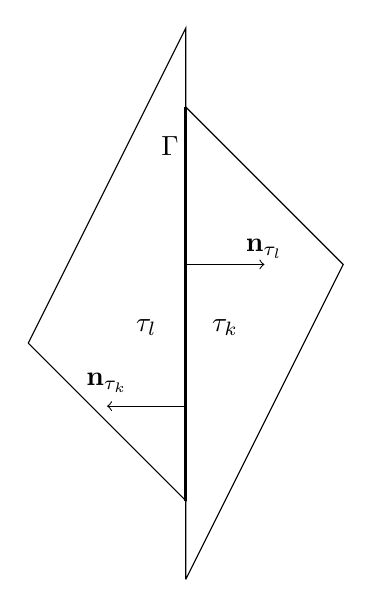
\begin{tikzpicture}
        \draw (0,2)--(2,0)--(2,6)--(0,2);
        \draw (2,-1)--(2,5)--(4,3)--(2,-1);
        \draw[line width=1pt] (2,0) -- (2,5);
        \draw[->] (2,3)--(3,3); 
        \draw[->] (2,1.2)--(1,1.2); 
        \node at (3,3.2) {$\textbf{n}_{\tau_l}$};
        \node at (1,1.5) {$\textbf{n}_{\tau_k}$};
        \node at (1.8,4.5) {$\Gamma$};
        \node at (1.5,2.2) {$\tau_l$};
        \node at (2.5,2.2) {$\tau_k$};
    \end{tikzpicture}
\end{center}
其中$\textbf{n}_{\tau_l}$为单元$\tau_l$向外的单位法向量,$\textbf{n}_{\tau_k}$为单元$\tau_k$向外的单位法向量。

随后我们有一些和间断有限元相似的定义,但仍然有些不同:

\begin{definition}[Jump and average]\label{def}.\\
    跳量和平均
    1.在内切面 $e_{kl}$ 上的跳量定义为:
    $$[v]_{e_{k l}}:=v|_{\tau_{k}} \boldsymbol{n}_{k}+v|_{\tau_{l}} \boldsymbol{n}_{l} $$
    更具体来说,在内切面 $e_{kl}$ 上空间方向的跳量定义为
    $$[v]_{e_{k l}, \boldsymbol{x}}:=v|_{\tau_{k}} n_{k, \boldsymbol{x}}+v|_{\tau_{l}} n_{l, \boldsymbol{x}} ,$$
    时间方向的跳量为:
    $$[v]_{e_{k l}, t}:=v|_{\tau_{k}} n_{k, t}+v|_{\tau_{l}} n_{l, t}  .$$
    2.函数v在内切面  $e_{kl}$ 上定义的平均量为:
    $$\langle v\rangle_{e_{kl}}:=\frac{1}{2}\left(v|_{\tau_{k}}+v|_{\tau_{l}}\right) ,$$
    3.在时间方向的迎风量为:
    $$\{v\}_{e_{k l}}^{\text {up }}:=\left\{\begin{array}{ll}
        v|_{ \tau_{k}} & \text { for } n_{k, t}>0 \\
        0 & \text { for } n_{k, t}=0 \\
        v|_{ \tau_{l}} & \text { for } n_{k, t}<0
        \end{array}  .\right.$$
    4.时间方向的顺风量为:
    $$\{v\}_{e_{k l}}^{\text {down }}:=\left\{\begin{array}{ll}
        v|_{ \tau_{l}} & \text { for } n_{k, t}>0 \\
        0 & \text { for } n_{k, t}=0 \\
        v|_{ \tau_{k}} & \text { for } n_{k, t}<0
        \end{array}  .\right.$$
\end{definition}

在这里 $\textbf{n}_k$ 为单元 $\tau_k$边上的单位法向量。其中 $n_x=\textbf{n}_k\cdot \hat{x}, n_t=\textbf{n}_k\cdot \hat{t}$,$\hat{x},\hat{t}$分别代表空间和时间方向的单位向量。
并且我们注意到对于在边界上的边 $e_{kl}\in \mathscr{E}_h^D,[v]=\{v\}=v$, 属于内部边的内切面 $e\in \mathscr{E}_h^I$,有$[vw]=[v]\{w\}+\{v\}[w]$

\subsubsection*{变分形式}

我们有弱解形式如下:

\begin{equation}
    \int_Qu_tv-\int_Q\Delta uv = \int_Q fv
\end{equation}

因此我们用内罚间断伽辽金方法来逼近拉普拉斯算子$\Delta u$,这里和利用DGM求解Possion方程类似,但由于时间维度的加入,推导变得复杂:

\begin{equation}\label{auv}
    \begin{aligned}
        a\left(u_{h}, v_{h}\right):=  &\sum_{l=1}^{N} \int_{\tau_{l}} \nabla_{x} u_{h} \cdot \nabla_{\boldsymbol{x}} v_{h} 
         -\sum_{e_{k l} \in \mathscr{E}_h^{ID}} \int_{e_{k l}}\left\langle\nabla_{\boldsymbol{x}} u_{h}\right\rangle_{e_{k l}} \cdot\left[v_{h}\right]_{e_{k l}, \boldsymbol{x}} \mathrm{d} s \\
        & +\epsilon\sum_{e_{k l} \in \mathscr{E}_h^{ID}} \int_{e_{k l}}\left[u_{h}\right]_{e_{k l}, \boldsymbol{x}} \cdot\left\langle\nabla_{\boldsymbol{x}} v_{h}\right\rangle_{e_{k l}} \mathrm{d} s \\
        & +\sum_{e_{k l} \in \mathscr{E}_h^{ID}} \frac{\sigma}{\overline{h_{k l}}} \int_{e_{k l}}\left[u_{h}\right]_{e_{k l}, \boldsymbol{x}} \cdot\left[v_{h}\right]_{e_{k l}, \boldsymbol{x}} \mathrm{d} s\\
    \end{aligned}
\end{equation}
注意第三项和第四项分别为添加的对称项和惩罚项。

对于时间导数,我们由格林公式可得:
$$\int_{\partial \tau}uv \cdot n_t ds = \int_\tau (u_tv+uv_t)d\tau$$

注意到在$\Sigma_D$上$n_t=0$, 那么我们可以逼近 $u_t$ 通过

\begin{equation}\label{buv}
    \begin{aligned}
        b\left(u_{h}, v_{h}\right):= &-\sum_{l=1}^{N} \int_{\tau_{l}} u_{h} \partial_{t} v_{h} +\int_{\Sigma_{T}} u_{h} v_{h} \cdot n_t ds  
         +\sum_{e_{k l} \in \mathscr{E}_h^{I}}\int_{e_{k l}}\left\{u_{h}\right\}_{e_{k l}}^{\mathrm{up}}\left[v_{h}\right]_{e_{k l}, t} ds
    \end{aligned}
\end{equation}

因此由 \hyperref[Interior Penalty Discontinuous Galerkin Method]{IPDG}, 问题可以转化为: 

\begin{tcolorbox}
寻找 $u_h\in S_h^p(Q_h)$ s.t.

$$A\left(u_{h}, v_{h}\right)=\left\langle f, v_{h}\right\rangle_{Q}+\left\langle u_{0}, v_{h}\right\rangle_{\Sigma_{0}}+\left\langle g, v_{h}\right\rangle_{\Sigma_{N}}$$
对于任意的  $v_{h} \in S_{h}^{p}\left(Q_h\right) $.

其中
$A\left(u_{h}, v_{h}\right):=a\left(u_{h}, v_{h}\right)+b\left(u_{h}, v_{h}\right)$
\end{tcolorbox}


那么我们可以定义$S_h^p(Q_h)$的基函数 $span\{\phi_k\}_{k=1}^M$,i.e.
$$S_h^p(Q_h)=span\{\phi_k\}_{k=1}^M,u_h(x,t)=\sum_{j=1}^{M}u_j\phi_j(x,t)\qquad u_h\in S_h^p(Q_h)$$


可以写成矩阵形式 $$A_hu=f$$ 其中 $A_h=A(\phi_j,\phi_i),f_i=\left\langle f, \phi_i\right\rangle_{Q}+\left\langle u_{0}, \phi_i\right\rangle_{\Sigma_{0}}+\left\langle g, \phi_i\right\rangle_{\Sigma_{N}}$

\section{STFEM for NS}

在热方程之后,我们再考虑NS方程。因此首先利用混合有限元方法进行解耦速度和压力。

\subsection{混合有限元方法(Mixed Finite Element Method)}
我们在变量耦合的地方应用MFEM。斯托克斯方程是NS方程雷诺数趋向于0的特殊情况,因此我们以斯托克斯方程作为例子。
$$\left\{
\begin{aligned}
    &-\Delta \textbf{u}+\nabla p = \textbf{f} \qquad &in\ \Omega\\
    &u=0\qquad &on \ \Gamma_D\\
    &\nabla \cdot \textbf{u} = 0\qquad &\Gamma_N\\
\end{aligned}
\right.$$
其中 $\textbf{u}=(u_1,u_2)$ 为速度场中向量, p 为压力场为标量, $\textbf{f}=(f_1, f_2)$。这里的困难在与如何解耦u和p这两个变量。
% As we can see, if some $(\textbf{u}, p)$ solve the equations above then $(\textbf{u}, p)$ does as well. 
为了解的唯一性,我们需要施加额外条件 $\int_\Omega p=0$

因此我们可以得到斯托克斯方程的弱形式: 寻找$\textbf{u}\in V=[H^1_0]^2$ 并且 $p\in W=L^2_0$ s.t.

$$\left\{
    \begin{aligned}
        &a(\textbf{u},\textbf{v})-b(\textbf{v}, p)=(\textbf{f}, \textbf{v}) \qquad &\forall \textbf{v}\in V\\
        &b(\textbf{u}, q)=0 \qquad &\forall q\in W
    \end{aligned}
\right.$$
其中 $$\begin{aligned}
    &a(\textbf{u},\textbf{v})=(\nabla \textbf{u},\nabla \textbf{v})=\int_\Omega \nabla \textbf{u}:\nabla \textbf{v}d\Omega\\
    &b(\textbf{v}, q)=(\nabla\cdot \textbf{v}, q)=\int_\Omega \nabla\cdot \textbf{v}\cdot q
\end{aligned}$$

\subsubsection{优化}
我们可以把上述问题转化为一个优化问题

\begin{tcolorbox}
    $$\begin{aligned}
    \textbf{u}&=arg \min_{\textbf{v}\in V, \nabla \cdot \textbf{v}=0}\left\{\frac{1}{2}\left\|\nabla \textbf{v}\right\|^2_{L^2(\Omega)}-(\textbf{f}, \textbf{v})\right\}\\
    &=arg \min_{\textbf{v}\in V} \max_{q\in W}\left\{\frac{1}{2}\left\|\nabla \textbf{v}\right\|^2_{L^2(\Omega)}-(\textbf{f}, \textbf{v}) -(\nabla \cdot \textbf{v}, q)\right\}
\end{aligned}$$
\end{tcolorbox}


\subsubsection*{注:}
这里min-max的形式自然形成对抗的形式,很自然的可以参考弱对抗神经网络(WAN)进行处理。因此我认为弱对抗神经网络是是处理弱解形式耦合问题好的方法(原本的弱对抗神经网络的关注点在于处理高维PDE)。

\subsubsection{离散化}

我们引入 $V_h\subset V, W_h\subset W$ 并且想要寻找$V_h$基函数 $\{\phi_1,\phi_2\cdots \phi_n\}$,  $W_h$中基函数$\{\psi_1, \psi_2\cdots \psi_m\}$. 
因此我们需要
\begin{tcolorbox}
    寻找 $(\textbf{u}_h, p_h)\in V_h\times W_h$, 更具体的是, $\textbf{u}_h=\sum_i\textbf{U}(\textbf{x}_i)\phi_i$ 和 $p=\sum_iP(\textbf{x}_i)\psi_i$ s.t. 

$$\left\{
\begin{aligned}
    &a(\textbf{u}^h, \textbf{v}^h)-b(\textbf{v}^h,p^h)=(\textbf{f}, \textbf{v}) \qquad &\forall \textbf{v}^h\in V_h\\
    &b(\textbf{u}^h, q^h)=0\qquad &\forall q\in W^h
\end{aligned}
\right.$$
\end{tcolorbox}


因此我们得到
$$\left\{
    \begin{aligned}
        &AU-BP=F\\
        &B^TU=0
    \end{aligned}
\right.\quad\text{i.e.}\quad 
\begin{pmatrix}
    A & -B\\
    B^T & 0
\end{pmatrix}\begin{pmatrix}
    U\\P
\end{pmatrix}=\begin{pmatrix}
    F\\0
\end{pmatrix}$$
其中 $A=(a_{ij}),a_{ij}=a(\phi_i, \phi_j)=(\nabla \phi_i, \nabla \phi_j);B=(b_{ij}),b_{ij}=b(\phi_j, \psi_i)=(\psi_i, \nabla\cdot\phi_j);F=(F_i),F_i=(\textbf{f},\phi_i)$

这是解决斯托克斯方程的混合有限元方法,它一个和时间无关的静态方程,然而对于真实的NS方程是瞬态方程。所以如何处理时间变量是一个重要的问题,这在上一节已经讨论过两种方法,下面展示时空方法。


\subsection{STDGM for NS}
在考虑热方程之后, 我们考虑NS方程的时空有限元方法。首先有方程:
$$\left\{
\begin{aligned}
    &\partial_{t} \boldsymbol{u}-v \Delta \boldsymbol{u}+\left(\boldsymbol{u} \cdot \nabla_{\boldsymbol{x}}\right) \boldsymbol{u}+\nabla_{\boldsymbol{x}} p  =\boldsymbol{f} & & \text { in } Q, \\
    &\nabla \cdot(\boldsymbol{u})  =0 & & \text { in } Q, \\
    &\boldsymbol{u}  =\boldsymbol{g}_{D} & & \text { on } \Sigma_{D}, \\
    &v\left(\nabla_{\boldsymbol{x}} \boldsymbol{u}\right) \boldsymbol{n}_{x}-p \boldsymbol{n}_{x}  =\mathbf{0} & & \text { on } \Sigma_{N}, \\
    &\boldsymbol{u}  =\boldsymbol{u}_{0} & & \text { on } \Sigma_{0} .
\end{aligned}\right.$$

定义函数空间
$$\left\{\begin{aligned}
    &V_{h}^{p+1}\left(Q_h\right) :=\left[S_{h}^{p+1}\left(Q_h\right)\right]^{d} 
    =\left\{\boldsymbol{v}_{h} \in\left[L_{2}(Q)\right]^{d}: \boldsymbol{v}_h|_{\tau_{l}} \in\left[\mathbb{P}_{p+1}\left(\tau_{l}\right)\right]^{d} \text { for all } \tau_{l} \in Q_h, \boldsymbol{v}_{h}=\mathbf{0} \text { on } \Sigma_{D}\right\} \\
    &W_{h}^{p}\left(Q_h\right) :=\left\{q_{h} \in L_{2}(Q): q_h|_{\tau_{l}} \in \mathbb{P}_{p}\left(\tau_{l}\right) \text { for all } \tau_{l} \in Q_h\right\} .
\end{aligned}\right.$$

首先式子中有热方程中的两项$\partial_{t} \boldsymbol{u}-v \Delta \boldsymbol{u}$,可以利用上述热方程的推导过程化为
$A\left(u_{h}, v_{h}\right):=a\left(u_{h}, v_{h}\right)+b\left(u_{h}, v_{h}\right)$,这里和热方程一样。

接下来我们考虑如何处理压力项的梯度$\nabla_x p$。我们同样有弱形式,并通过分部积分写成跳量形式可以得到:

$$\begin{aligned}
    &-\int_{Q} \nabla_{\boldsymbol{x}} p \cdot \boldsymbol{v}_{h}  \\=& -\sum_{\ell=1}^{N} \int_{\tau_{\ell}} \nabla_{\boldsymbol{x}} p \cdot \boldsymbol{v}_{h}  
    =  \sum_{\ell=1}^{N} \int_{\tau_{\ell}} p \nabla_x \cdot{v}_{h} -\sum_{\ell=1}^{N} \int_{\partial \tau_{\ell}} p \boldsymbol{v}_{h} \cdot \boldsymbol{n}_{\boldsymbol{x}} \mathrm{d} s\\
    = & \sum_{\ell=1}^{N} \int_{\tau_{\ell}} p \nabla_x \cdot{v}_{h} -\int_{\Sigma_{N}} p \boldsymbol{v}_{h} \cdot \boldsymbol{n}_{\boldsymbol{x}} \mathrm{d} s-\left\langle\boldsymbol{u}_{0}, \boldsymbol{v}_{h}\right\rangle_{\Sigma_{0}}
     -\sum_{\Gamma_{k \ell} \in \mathscr{E}_{h}^I} \int_{\Gamma_{k \ell}}\left[p \boldsymbol{v}_{h}\right]_{\Gamma_{k \ell}, \boldsymbol{x}} \mathrm{d} s\\
     = & \sum_{\ell=1}^{N} \int_{\tau_{\ell}} p \nabla_x \cdot{v}_{h} -\int_{\Sigma_{N}} p \boldsymbol{v}_{h} \cdot \boldsymbol{n}_{\boldsymbol{x}} \mathrm{d} s
     -\sum_{\Gamma_{k \ell} \in \mathscr{E}_{h}^I} \int_{\Gamma_{k \ell}}\langle p \rangle_{\Gamma_{k \ell}}[\boldsymbol{v}_{h}]_{\Gamma_{k \ell}, \boldsymbol{x}} \mathrm{d} s-\left\langle\boldsymbol{u}_{0}, \boldsymbol{v}_{h}\right\rangle_{\Sigma_{0}}
\end{aligned}$$

因此我们可以定义双线性型
$$B(v_h, p_h)=\sum_{\ell=1}^{N} \int_{\tau_{\ell}} p_h \nabla_x \cdot{v}_{h} -\sum_{\Gamma_{k \ell} \in \mathscr{E}_{h}^I} \int_{\Gamma_{k \ell}}\langle p_h \rangle_{\Gamma_{k \ell}}[\boldsymbol{v}_{h}]_{\Gamma_{k \ell}, \boldsymbol{x}} \mathrm{d} s$$

根据混合有限元方法, 可以得到$B(u_h, q_h)=0\quad \forall q_h\in W_{h}^{p}\left(Q_h\right)$,并且用该式子代替$\nabla \cdot u=0$。

同时我们给压力项添加稳定项
$$D\left(p_{h}, q_{h}\right):=\sigma_{p} \sum_{\Gamma_{k \ell} \in \mathcal{I}_{N}} \bar{h}_{k \ell} \int_{\Gamma_{k \ell}}\left[p_{h}\right]_{\Gamma_{k \ell}}(\boldsymbol{x}, t) \cdot\left[q_{h}\right]_{\Gamma_{k \ell}}(\boldsymbol{x}, t) \mathrm{d} s_{(\boldsymbol{x}, t)}$$

问题变成:
\begin{tcolorbox}
寻找 $\boldsymbol{u}_{h}=\boldsymbol{u}_{h, 0}+\mathcal{E} \boldsymbol{g}_{D}$ 其中 $\boldsymbol{u}_{h, 0} \in V_{h}^{p+1}\left(Q_h\right)$和 $p_{h} \in W_{h}^{p}\left(Q_h\right)$, s.t.

$$\begin{aligned}
A\left(\boldsymbol{u}_{h}, \boldsymbol{v}_{h}\right)+\left\langle\left(\boldsymbol{u}_{h} \cdot \nabla_{\boldsymbol{x}}\right) \boldsymbol{u}_{h}, \boldsymbol{v}_{h}\right\rangle_{Q}-B\left(\boldsymbol{v}_{h}, p_{h}\right) & =\left\langle\boldsymbol{f}, \boldsymbol{v}_{h}\right\rangle_{Q}+\left\langle\boldsymbol{u}_{0}, \boldsymbol{v}_{h}\right\rangle_{\Sigma_{0}}, \\
B\left(\boldsymbol{u}_{h}, q_{h}\right)+D\left(p_{h}, q_{h}\right) & =0
\end{aligned}$$

对于任意 $\boldsymbol{v}_{h} \in V_{h}^{p+1}\left(Q_h\right)$,  $q_{h} \in W_{h}^{p}\left(Q_h\right)$ 
\end{tcolorbox}


同时对于离散化函数空间,我们定义基函数
$$\left\{\begin{aligned}
    &V_{h}^{p+1}\left(Q_h\right)=\operatorname{span}\left\{\boldsymbol{\varphi}_{l=1}\right\}_{l}^{M_{u}}, \qquad& \boldsymbol{u}_{h, 0}=\sum_{l=1}^{M_{u}} \boldsymbol{u}[l] \boldsymbol{\varphi}_{l} & \text { for } \boldsymbol{u}_{h, 0} \in V_{h}^{p+1}\left(Q_h\right) \\
    &W_{h}^{p}\left(Q_h\right)=\operatorname{span}\left\{\psi_{n}\right\}_{n=1}^{M_{p}}, \qquad & p_{h}=\sum_{n=1}^{M_{p}} \boldsymbol{p}[n] \psi_{n} & \text { for } p_{h} \in W_{h}^{p}\left(Q_h\right)
\end{aligned}\right.$$

基于此我们定义非线性算子
$$\left(K_{h} \boldsymbol{u}\right)[k]:=A\left(\boldsymbol{u}_{h}, \boldsymbol{\varphi}_{k}\right)+\left\langle\left(\boldsymbol{u}_{h} \cdot \nabla_{\boldsymbol{x}}\right) \boldsymbol{u}_{h}, \boldsymbol{\varphi}_{k}\right\rangle_{Q}$$

其中$\boldsymbol{u}_{h}=\mathcal{E} \boldsymbol{g}_{D}+\sum_{l=1}^{M_{u}} \boldsymbol{u}[l] \boldsymbol{\varphi}_{l}$ 

以及$B_{h}[m, l]:=B\left(\varphi_{l}, \psi_{m}\right), \quad D_{h}[m, n]:=D\left(\psi_{n}, \psi_{m}\right)$,其中$k, l=1, \ldots, M_{u}$, $m, n=1, \ldots, M_{p}$. 

可以得到矩阵形式
$$\left(\begin{array}{cc}
K_{h} & -B_{h}^{\top} \\
B_{h} & D_{h}
\end{array}\right)\left(\begin{array}{l}
\boldsymbol{u} \\
\boldsymbol{p}
\end{array}\right)=\left(\begin{array}{l}
\boldsymbol{f}_{u} \\
\boldsymbol{f}_{p}
\end{array}\right)$$

可以看到由于 $u_h$ 未知,方程中的非线性项非常难处理, 在这里我们可以通过牛顿迭代的方法处理。当然随着深度学习在各个领域的发展,在非线性优化方面也显现出很大的潜力。

\section{关于多尺度问题}
当离散化空间非常大的时候,有比较将区域进行分解,例如可以对于微观和宏观的区域可以各自进行不同的离散化策略。然而对于区域分解来说,困难在于边界处如何耦合的问题。
因此在这里提出混合离散的方式,考虑针对有多尺度的问题。

\subsection{混合离散}
我们通过将区域分解成多个小区域,并且对于不同的区域可以采取不同的离散化方案。因此,对于无论是空间还是时间上的多尺度问题我们都可以通过区域上的网格加密来实现。

首先说明区域的分解方案。我们提出将时空区域$Q$分解为子区域 $Q_i$, i.e.$Q=\cup_i^pQ_i$。如图\ref{subdomain}所示, 
且记 $\Sigma_i=\overline{\partial Q_i/\partial Q},\Sigma=\cup_i^p \Sigma_i$
可以看出 $\Sigma$ 为不同的子区域的交界面。对于不同的子区域$Q_i$我们有不同的分解: $Q_i=\mathscr{T}_{N_i}:=\cup_{l=1}^{N_i}\tau_l^i$. 

因此有
$$\left\{
    \begin{aligned}
        \overline{Q}&=\overline{\mathscr{T}_N}=\cup_{i=1}^p\overline{\mathscr{T}_{N_i}}=\cup_i^p\cup_l^{N_i}\overline{\tau_l^i}\\
        \Sigma_h&=\mathscr{E}_N^I/ \cup_i^p\mathscr{E}_{N_i}^I
    \end{aligned}\right.$$
在这里我们将 $\mathscr{E}_N^I$记作$\mathcal{I}_N$.

\begin{figure}[H]
    \begin{center}
        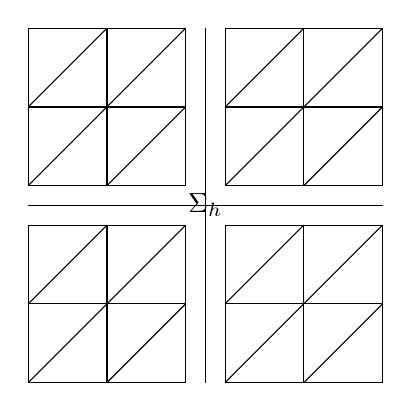
\begin{tikzpicture}  
            \foreach \m in {0,2.5}
            {\foreach \n in {0,2.5}
            {\draw (0+\n,0+\m) -- (2+\n,0+\m);  
            \draw (0+\n,1+\m) -- (2+\n,1+\m);  
            \draw (0+\n,2+\m) -- (2+\n,2+\m);  
            \draw (0+\n,0+\m) -- (0+\n,2+\m); 
            \draw (1+\n,0+\m) -- (1+\n,2+\m);  
            \draw (2+\n,0+\m) -- (2+\n,2+\m);  
    
            \foreach \y in {0,1}  
            {  
                \draw (\y+\n,0+\m) -- (2+\n,2-\y+\m);
            }  
            \foreach \y in {1,2}  
            {  
                \draw (0+\n,\y+\m) -- (2-\y+\n,2+\m);   
            } } }
    
            \draw (0, 2.25)--(4.5,2.25);
            \draw (2.25, 4.5)--(2.25,0);
            \node at (2.25,2.25) {$\Sigma_h$}; 
        \end{tikzpicture} 
    \end{center}
    \caption{Subdomains}
    \label{subdomain}
\end{figure}

同时我们定义离散化函数空间 $$S_h^p(\Sigma_h)=\{v_h\in L_2(\Sigma):v_h|_{\Gamma_{kl}}\in P_p(\Gamma_{kl}),\forall \Gamma_{kl}\in \Sigma_h\}$$

为了书写时下标不至于太多,在这里我们同样以前面简单的热方程为例,介绍其理论: 

对于整个区域上写成弱形式,同之前介绍的理论,即寻找$u_h \in S_h^p(\mathscr{T}_N)$ s.t.$\forall v_h\in S_h^p(\mathscr{T}_N)$, 
$$A(u_h,v_h)=\langle f,v_h\rangle_Q+\langle u_0,v_h\rangle_{\Sigma_0}+\langle g_N,v_h\rangle_{\Sigma_N}$$ 

那么我们可以分别将该方案应用到 $Q_i$ 上。因此我们有局部的双线性型: 其中 $u_h^i,v_h^i \in S_h^p(\mathscr{T}_{N_i})$ s.t. 对于  $i=1, \ldots, P$
$$A^{(i)}(u_h^i, v_h^i):=a^{(i)}(u_h^i,v_h^i)+b^{(i)}(u_h^i,v_h^i)=F^{(i)}\left(v_{h}^{i}\right)$$
其中
\begin{equation}\label{hybrid}\left\{\begin{aligned}
    a^{(i)}(u_h^i,v_h^i)&=\sum_{l=1}^{N_i}\int_{\tau_l^i}\nabla_x u_h^i\cdot \nabla_x v_h^i d\tau\\
    &-\sum_{\Gamma_{k l} \in \mathcal{I}_{N_{i}}} \int_{\Gamma_{k l}}\left(\left\langle\nabla_{\boldsymbol{x}} u_{h}^{i}\right\rangle_{\Gamma_{k l}} \cdot\left[v_{h}^{i}\right]_{\Gamma_{k l}, \boldsymbol{x}} + \left[u_{h}^{i}\right]_{\Gamma_{k l}, \boldsymbol{x}} \cdot\left\langle\nabla_{\boldsymbol{x}} v_{h}^{i}\right\rangle_{\Gamma_{k l}}\right) \mathrm{d} s \\
    &+\sum_{\Gamma_{k l} \in \mathcal{I}_{N_{i}}} \frac{\sigma}{\overline{h_{k l}}} \int_{\Gamma_{k l}}\left[u_{h}^{i}\right]_{\Gamma_{k l}, \boldsymbol{x}} \cdot\left[v_{h}^{i}\right]_{\Gamma_{k l}, \boldsymbol{x}} \mathrm{d} s\\
    b^{(i)}\left(u_{h}^{i}, v_{h}^{i}\right)&= -\sum_{l=1}^{N_{i}} \int_{\tau_{l}^{i}} u_{h}^{i} \partial_{t} v_{h}^{i} +\int_{\Sigma_{T} \cap \partial Q_{i}} u_{h}^{i} v_{h}^{i} \mathrm{d} s 
     +\sum_{\Gamma_{k l} \in \mathcal{I}_{N_{i}} }\int_{\Gamma_{k l}}\left\{u_{h}^{i}\right\}_{\Gamma_{k l}}^{\mathrm{up}}\left[v_{h}^{i}\right]_{\Gamma_{k l}, t} \mathrm{d} s\\
    F^{(i)}\left(v_{h}^{i}\right)&=\left\langle f, v_{h}^{i}\right\rangle_{Q_{i}}+\left\langle u_{0}, v_{h}^{i}\right\rangle_{\Sigma_{0} \cap \partial Q_{i}}+\left\langle g_{N}, v_{h}^{i}\right\rangle_{\Sigma_{N} \cap \partial Q_{i}},
\end{aligned}\right.\end{equation}


由于  $u_{h}^{i}=u_{h}|_{Q_{i}}$, 因此我们可以将整个区域上的双线性型$A(\cdot, \cdot)$分解成局部的双线性型$A^{(i)}(\cdot, \cdot)$的和以及区域交界面$\Sigma_{h}$上的耦合部分。 

即:
\begin{equation}\label{Hybrid}\begin{aligned}
    A\left(u_{h}, v_{h}\right)= & \sum_{i=1}^{P} A^{(i)}\left(u_{h}, v_{h}\right)
    -\sum_{\Gamma_{k l} \in \Sigma_{h}} \int_{\Gamma_{k l}}\left(\left\langle\nabla_{\boldsymbol{x}} u_{h}\right\rangle_{\Gamma_{k l}} \cdot\left[v_{h}\right]_{\Gamma_{k l}, \boldsymbol{x}} +\left[u_{h}\right]_{\Gamma_{k l}, \boldsymbol{x}} \cdot\left\langle\nabla_{\boldsymbol{x}} v_{h}\right\rangle_{\Gamma_{k l}}\right)\mathrm{d} s \\
    & +\sum_{\Gamma_{k l} \in \Sigma_{h}} \frac{\sigma}{\bar{h}_{k l}} \int_{\Gamma_{k l}}\left[u_{h}\right]_{\Gamma_{k l}, \boldsymbol{x}} \cdot\left[v_{h}\right]_{\Gamma_{k l}, \boldsymbol{x}} \mathrm{d} s +\sum_{\Gamma_{k l} \in \Sigma_{h}} \int\left\{u_{h}\right\}_{\Gamma_{k l}}^{\mathrm{up}}\left[v_{h}\right]_{\Gamma_{k l}, t} \mathrm{d} s .
\end{aligned}\end{equation}

为了减少交界面 $\Sigma$上的耦合量, 在交界面 $\Sigma$上定义如下新的变量:$\lambda_h\in S_h^p(\Sigma_h)$: $\lambda_h|_{\tau_{kl}}=\frac{1}{2}(u_h|_{\tau_k}+u_h|_{\tau_l})$。

同时我们有如下新记号:
\begin{definition}[Hybrid Jump]
    $$[u/\lambda]_{\partial \tau_k}=(u|_{\tau_k}-\lambda)\textbf{n}_k$$
\end{definition}

那么自然的可以推导出如下性质 $$[u]_{\Gamma_{kl}}=2[u/\lambda]_{\partial \tau_k}=2[u/\lambda]_{\partial \tau_l}$$ 
且 $$[u_h]_{\Gamma_{kl},x}\cdot \langle\nabla_x v_h\rangle=[u_h/\lambda_h]_{\partial \tau_k,x}\cdot\nabla v_h|_{\tau_k}+[u_h/\lambda_h]_{\partial \tau_l,x}\cdot\nabla v_h|_{\tau_l}$$

因此 
$$\begin{aligned}
    &\sum_{\Gamma_{k l} \in \Sigma_{h}} \int_{\Gamma_{k l}}\left[u_{h}\right]_{\Gamma_{k l}, \boldsymbol{x}} \cdot\left\langle\nabla_{\boldsymbol{x}} v_{h}\right\rangle_{\Gamma_{k l}} \mathrm{d} s\\
    =&\sum_{\Gamma_{k l} \in \Sigma_{h}}\int_{\Gamma_{k l}}\left(\left[u_{h} / \lambda_{h}\right]_{\partial \tau_{k}, \boldsymbol{x}} \cdot \nabla_{\boldsymbol{x}} v_{h }|_{\tau_{k}}+\left[u_{h} / \lambda_{h}\right]_{\partial \tau_{l}, \boldsymbol{x}} \cdot \nabla_{\boldsymbol{x}} v_{h }|_{\tau_{l}}\right) \mathrm{d} s \\
    =&\sum_{i=1}^{P} \sum_{l=1}^{N_{i}} \sum_{\substack{\Gamma_{k l} \in \Sigma_{h} \\\Gamma_{k l} \subset \partial \tau_{l}^{i} }}\int_{\Gamma_{k l}}\left[u_{h} / \lambda_{h}\right]_{\partial \tau_{l}^{i}, \boldsymbol{x}} \cdot \nabla_{\boldsymbol{x}} v_{h }|_{\tau_{l}^{i}} \mathrm{d} s .
\end{aligned}$$

同理,我们可以定义关于测试函数$v_h$的新变量 $\mu_h=\frac{1}{2}(v_h|_{\tau_k}+v_h|_{\tau_l})\in S_h^p(\Sigma_h)$ , 因此对称项变为
$$\sum_{\Gamma_{k l} \in \Sigma_{h}} \int_{\Gamma_{k l}}\left\langle\nabla_{\boldsymbol{x}} u_{h}\right\rangle_{\Gamma_{k l}} \cdot\left[v_{h}\right]_{\Gamma_{k l}, \boldsymbol{x}} \mathrm{d} s= \\
    \sum_{i=1}^{P} \sum_{l=1}^{N_{i}} \sum_{\substack{\Gamma_{k l} \in \Sigma_{h} \\
    \Gamma_{k l} \subset \partial \tau_{l}^{i}}} \int_{\Gamma_{k l}} \nabla_{\boldsymbol{x}} u_{h }|_{\tau_{l}^{i}}\cdot\left[v_{h} / \mu_{h}\right]_{\partial \tau_{l}^{i}, \boldsymbol{x}} \mathrm{d} s . \\$$

同时我们注意到 
$${\left[u_{h}\right]_{\Gamma_{k l}, \boldsymbol{x}} \cdot\left[v_{h}\right]_{\Gamma_{k l}, \boldsymbol{x}}}    
    =2\left[u_{h} / \lambda_{h}\right]_{\partial \tau_{k}, \boldsymbol{x}} \cdot\left[v_{h} / \mu_{h}\right]_{\partial \tau_{k}, \boldsymbol{x}}
    +2\left[u_{h} / \lambda_{h}\right]_{\partial \tau_{l}, \boldsymbol{x}} \cdot\left[v_{h} / \mu_{h}\right]_{\partial \tau_{l}, \boldsymbol{x}}$$    
    
因此惩罚项可以写成
    
$$\begin{aligned}
&\sum_{\Gamma_{k l} \in \Sigma_{h}} \frac{\sigma}{\bar{h}}_{k l} \int_{\Gamma_{k l}}\left[u_{h}\right]_{\Gamma_{k l}, \boldsymbol{x}} \cdot\left[v_{h}\right]_{\Gamma_{k l}, \boldsymbol{x}} \mathrm{d} s \\
=&\sum_{\Gamma_{k l} \in \Sigma_{h}} \frac{2 \sigma}{\bar{h}_{k l}} \int_{\Gamma_{k l}}\left( {\left[u_{h} / \lambda_{h}\right]_{\partial \tau_{k}, \boldsymbol{x}} \cdot\left[v_{h} / \mu_{h}\right]_{\partial \tau_{k}, \boldsymbol{x}} }+\left[u_{h} / \lambda_{h}\right]_{\partial \tau_{l}, \boldsymbol{x}} \cdot\left[v_{h} / \mu_{h}\right]_{\partial \tau_{l}, \boldsymbol{x}}\right) \mathrm{d} s \\
=&\sum_{i=1}^{P} \sum_{l=1}^{N_{i}} \sum_{\substack{\Gamma_{k l} \in \Sigma_{h} \\
\Gamma_{k l} \subset \partial \tau_{l}^{i}}} \frac{2 \sigma}{\overline{h}} \int_{\Gamma_{k l}}\left[u_{h} / \lambda_{h}\right]_{\partial \tau_{l}^{i}, \boldsymbol{x}} \cdot\left[v_{h} / \mu_{h}\right]_{\partial \tau_{l}^{i}, \boldsymbol{x}} \mathrm{d} s .
\end{aligned}$$

关于在\ref{Hybrid}中涉及迎风变量的项,我们可以同样定义
\begin{definition}[Hybrid Upwind]
    $$\{u / \lambda\}_{\partial \tau_{k}}^{\operatorname{up}}(\boldsymbol{x}, t):=\left\{\begin{array}{ll}
        u|_{ \tau_{k}}(\boldsymbol{x}, t) & \text { for } n_{k, t} \geq 0, \\
        0 & \text { for } n_{k, t}=0, \\
        \lambda(\boldsymbol{x}, t) & \text { for } n_{k, t}<0
        \end{array} \quad \text { for }(\boldsymbol{x}, t) \in \Gamma_{k l} .\right.$$
\end{definition}

那么对于精确解我们有, $\lambda=\langle u\rangle_{\Gamma_{kl}}=u|_{\tau_k}=u|_{\tau_l}$, 则
$$\sum_{\Gamma_{k l} \in \Sigma_{h}} \int_{\Gamma_{k l}}\left\{u_{h}\right\}_{\Gamma_{k l}}^{\text {up }}\left[v_{h}\right]_{\Gamma_{k l}, t} \mathrm{d} s=\sum_{i=1}^{P} \sum_{l=1}^{N_{i}} \sum_{\substack{\Gamma_{k l} \in \Sigma_{h} \\
\Gamma_{k l} \subset \partial \tau_{l}^{i}}}\int_{\Gamma_{kl}}\{u_h/\lambda_h\}_{\partial \tau_l^i}^{up}[v_h/\mu_h]_{\partial \tau_l^i,x}ds$$

因此我们可以将\ref{Hybrid}中所有涉及耦合边界上的项写为
$$\begin{aligned}
    &C^{(i)}(u_h,\lambda_h;v_h,\mu_h)\\
    =&-\sum_{l=1}^{N_{i}} \sum_{\substack{\Gamma_{k l} \in \Sigma_{h} \\
    \Gamma_{k l} \subset \partial \tau_{l}^{i}}} \int_{\boldsymbol{l}} \nabla_{\boldsymbol{x} l} u_{h \mid \tau_{l}^{i}} \cdot\left[v_{h} / \mu_{h}\right]_{\partial \tau_{l}^{i}, \boldsymbol{x}} \mathrm{d} s \\
    &+\sum_{l=1}^{N_{i}} \sum_{\substack{\Gamma_{k l} \in \Sigma_{h} \\
    \Gamma_{k l} \subset \partial \tau_{l}^{i}}} \frac{2 \sigma}{\bar{h}_{k l}} \int_{\Gamma_{k l}}\left[u_{h} / \lambda_{h}\right]_{\partial \tau_{l}^{i}, \boldsymbol{x}} \cdot\left[v_{h} / \mu_{h}\right]_{\partial \tau_{l}^{i}, \boldsymbol{x}} \mathrm{d} s \\
    &+\sum_{\substack{l=1}}^{N_{i}} \sum_{\substack{\Gamma_{k l} \in \Sigma_{h} \\
    \Gamma_{k l} \subset \partial \tau_{l}^{i}}} \int_{k l}\left\{u_{h} / \lambda_{h}\right\}_{\partial \tau_{l}^{i}}^{\mathrm{up}}\left[v_{h} / \mu_{h}\right]_{\partial \tau_{l}^{i}, \boldsymbol{x}} \mathrm{d} s . \\
\end{aligned}$$

最终我们将问题转化为:
\begin{tcolorbox}
    求解 $u_h\in S_h^p(\mathscr{T}_h)\& \lambda_h\in S_h^p(\Sigma_h)$ s.t. for $\forall v_h\in S_h^p(\mathscr{T}_h)\& \mu_h\in S_h^p(\Sigma_h)$,
$$\sum_{i=1}^{p}\left[A^{(i)}(u_h,v_h)+C^{(i)}(u_h,\lambda_h;v_h,\mu_h)\right]=\sum_{i=1}^{p}F^{(i)}(v_h)$$
\end{tcolorbox}


对于每一个时空区域的离散,我们有
\begin{itemize}
    \item $\mathscr{T}_{N_i}=span\{\phi_l^i\}^{M_i}_l$, for $u_h^i\in S_h^p(\mathscr{T}_{N_i})$, 因此设 $u_h^i=\sum_{l=1}^{M_i}U_l^i\phi_l^i(x,t)$
    \item $S_h^p(\Sigma_h)=span\{\psi_n\}_{n=1}^{M_\Sigma}$, for $\lambda_h\in S_h^p(\Sigma_h)$, 因此设 $\lambda_h=\sum_{n=1}^{M_\Sigma}\lambda_\Sigma^n\psi_n(x,t)$
\end{itemize}

因此我们有线性形式

$$\left\{\begin{aligned}
    &A_{I I}^{(i)}[k, \ell]  =A^{(i)}\left(\varphi_{\ell}^{i}, \varphi_{k}^{i}\right)+C^{(i)}\left(\varphi_{\ell}^{i}, 0 ; \varphi_{k}^{i}, 0\right) & \text { for } k, \ell=1, \ldots, M_{i}, \\
    &A_{I \Sigma}^{(i)}[k, n]:=C^{(i)}\left(0, \psi_{n} ; \varphi_{k}^{i}, 0\right) & \text { for } k=1, \ldots, M_{i} \text { and } n=1, \ldots, M_{\Sigma} \\
    &A_{\Sigma I}^{(i)}[m, \ell]  :=C^{(i)}\left(\varphi_{\ell}^{i}, 0 ; 0, \psi_{m}\right) & \text { for } m=1, \ldots, M_{\Sigma} \text { and } \ell=1, \ldots, M_{i}\\
    &A_{\Sigma \Sigma}[m, n]:=\sum_{i=1}^{P} C^{(i)}\left(0, \psi_{n} ; 0, \psi_{m}\right) & \text { for } m, n=1, \ldots, M_{\Sigma} .
\end{aligned}\right.$$
    
右端项为
$$F_{I}^{(i)}[k]:=F^{(i)}\left(\varphi_{k}^{i}\right) \quad \text { for } k=1, \ldots, M_{i} .$$

\paragraph*{矩阵形式}
可以写成矩阵形式:
$$\left(\begin{array}{ccccc}
    A_{I I}^{(1)} & & & & A_{I \Sigma}^{(1)} \\
    & A_{I I}^{(2)} & & & A_{I \Sigma}^{(2)} \\
    & & \ddots & & \vdots \\
    & & & A_{I I}^{(P)} & A_{I \Sigma}^{(P)} \\
    A_{\Sigma I}^{(1)} & A_{\Sigma I}^{(2)} & \cdots & A_{\Sigma I}^{(P)} & A_{\Sigma \Sigma}
    \end{array}\right)\left(\begin{array}{c}
    \boldsymbol{u}_{I}^{(1)} \\
    \boldsymbol{u}_{I}^{(2)} \\
    \vdots \\
    \boldsymbol{u}_{I}^{(P)} \\
    \boldsymbol{\lambda}_{\Sigma}
    \end{array}\right)=\left(\begin{array}{c}
    \boldsymbol{f}_{I}^{(1)} \\
    \boldsymbol{f}_{I}^{(2)} \\
    \vdots \\
    \boldsymbol{f}_{I}^{(P)} \\
    \mathbf{0}
\end{array}\right) .$$

可以发现这类矩阵是超大型稀疏矩阵,因为每个子矩阵都是稀疏的,且子矩阵也是稀疏的。因此如何避免求解这种超大型稀疏矩阵我们在第三章进行探讨。
我们希望借助深度学习的力量来避免线性方程组的求解,以达到更快更准的目标。
